%%%%%%%%%%%%%%%%%%%%%%%%%%%%%%%%%%%%%%%%%
% Short Sectioned Assignment
% LaTeX Template
% Version 1.0 (5/5/12)
%
% This template has been downloaded from:
% http://www.LaTeXTemplates.com
%
% Original author:
% Frits Wenneker (http://www.howtotex.com)
%
% License:
% CC BY-NC-SA 3.0 (http://creativecommons.org/licenses/by-nc-sa/3.0/)
%
%%%%%%%%%%%%%%%%%%%%%%%%%%%%%%%%%%%%%%%%%

%----------------------------------------------------------------------------------------
%	PACKAGES AND OTHER DOCUMENT CONFIGURATIONS
%----------------------------------------------------------------------------------------

\documentclass[paper=a4, fontsize=11pt]{scrartcl} % A4 paper and 11pt font size

\usepackage[T1]{fontenc} % Use 8-bit encoding that has 256 glyphs
%\usepackage{fourier} % Use the Adobe Utopia font for the document - comment this line to return to the LaTeX default
\usepackage[english]{babel} % English language/hyphenation
\usepackage{amsmath,amsfonts,amsthm} % Math packages
\usepackage{mathtools} %More math! (For dscases)
\usepackage{hyperref} %HTML package
\usepackage{pgfplots} %Makes plots in LaTeX
\usepackage{tikz} %Also tikz?
\usepackage{bm} %makes vectors bold
\usepackage{bbm} %Blackboard bold 1
\usepgfplotslibrary{fillbetween}%Let's me fill between named plots
\usepackage{graphicx} %import pics

\usepackage[noend]{algpseudocode} %Algorithms
\usepackage{algorithm}

\graphicspath{ {Python\_figs/} }
\DeclareGraphicsExtensions{.pdf,.png,.jpg}
\usepackage{sectsty} % Allows customizing section commands
\allsectionsfont{ \normalfont\scshape} % Make all sections the default font and small caps


\renewcommand{\thesubsection}{\alph{subsection}} %Make subsections start with letters

\usepackage{fancyhdr} % Custom headers and footers
\pagestyle{fancyplain} % Makes all pages in the document conform to the custom headers and footers
\fancyhead{} % No page header - if you want one, create it in the same way as the footers below
\fancyfoot[L]{} % Empty left footer
\fancyfoot[C]{} % Empty center footer
\fancyfoot[R]{\thepage} % Page numbering for right footer
\renewcommand{\headrulewidth}{0pt} % Remove header underlines
\renewcommand{\footrulewidth}{0pt} % Remove footer underlines
\setlength{\headheight}{13.6pt} % Customize the height of the header

\numberwithin{equation}{section} % Number equations within sections (i.e. 1.1, 1.2, 2.1, 2.2 instead of 1, 2, 3, 4)
\numberwithin{figure}{section} % Number figures within sections (i.e. 1.1, 1.2, 2.1, 2.2 instead of 1, 2, 3, 4)
\numberwithin{table}{section} % Number tables within sections (i.e. 1.1, 1.2, 2.1, 2.2 instead of 1, 2, 3, 4)

\setlength\parindent{0pt} % Removes all indentation from paragraphs - comment this line for an assignment with lots of text
\usepackage{listings}
\lstset{language=Prolog}
\usepackage{tikz-qtree}

\usepackage{placeins}
\usepackage{tikz}
\usetikzlibrary{decorations.pathmorphing, shapes.multipart,calc, arrows, positioning}


%----------------------------------------------------------------------------------------
%	TITLE SECTION
%----------------------------------------------------------------------------------------

\newcommand{\horrule}[1]{\rule{\linewidth}{#1}} % Create horizontal rule command with 1 argument of height

\title{	Homework 4}

\author{Benjamin Jakubowski} % Your name

\date{\normalsize\today} % Today's date or a custom date

\begin{document}

\maketitle % Print the title

%----------------------------------------------------------------------------------------
%	PROBLEM 1
%----------------------------------------------------------------------------------------

\section{Garbage Collection}

\subsection{Heap pointer allocation method}

Assume the 'heap pointer' allocation method is used to allocate memory. We draw the contents of the heap upon entry into \texttt{BeginEventLoop}, but before any garbage collection has taken place, identifying and showing the address of each object in the heap. In addition, we show the address of the heap pointer at that moment (assuming heap memory begins at address 0 and that the heap pointer is incremented by the size of the allocated object during each allocation.) Note each object takes:
\begin{itemize}
\item \textbf{Car}: 24 bytes + 8 byte forwarding address = 32 bytes
\item \textbf{Wheel}: 12 bytes + 8 byte forwarding address = 20 bytes
\item \textbf{Carwash}: 32 bytes + 8 byte forwarding address = 40 bytes
\item \textbf{Garage}: 32 bytes + 8 byte forwarding address = 40 bytes
\item \textbf{EventLog}: 8 bytes + 8 byte forwarding address = 16 bytes
\end{itemize}

\begin{center}
\begin{figure}
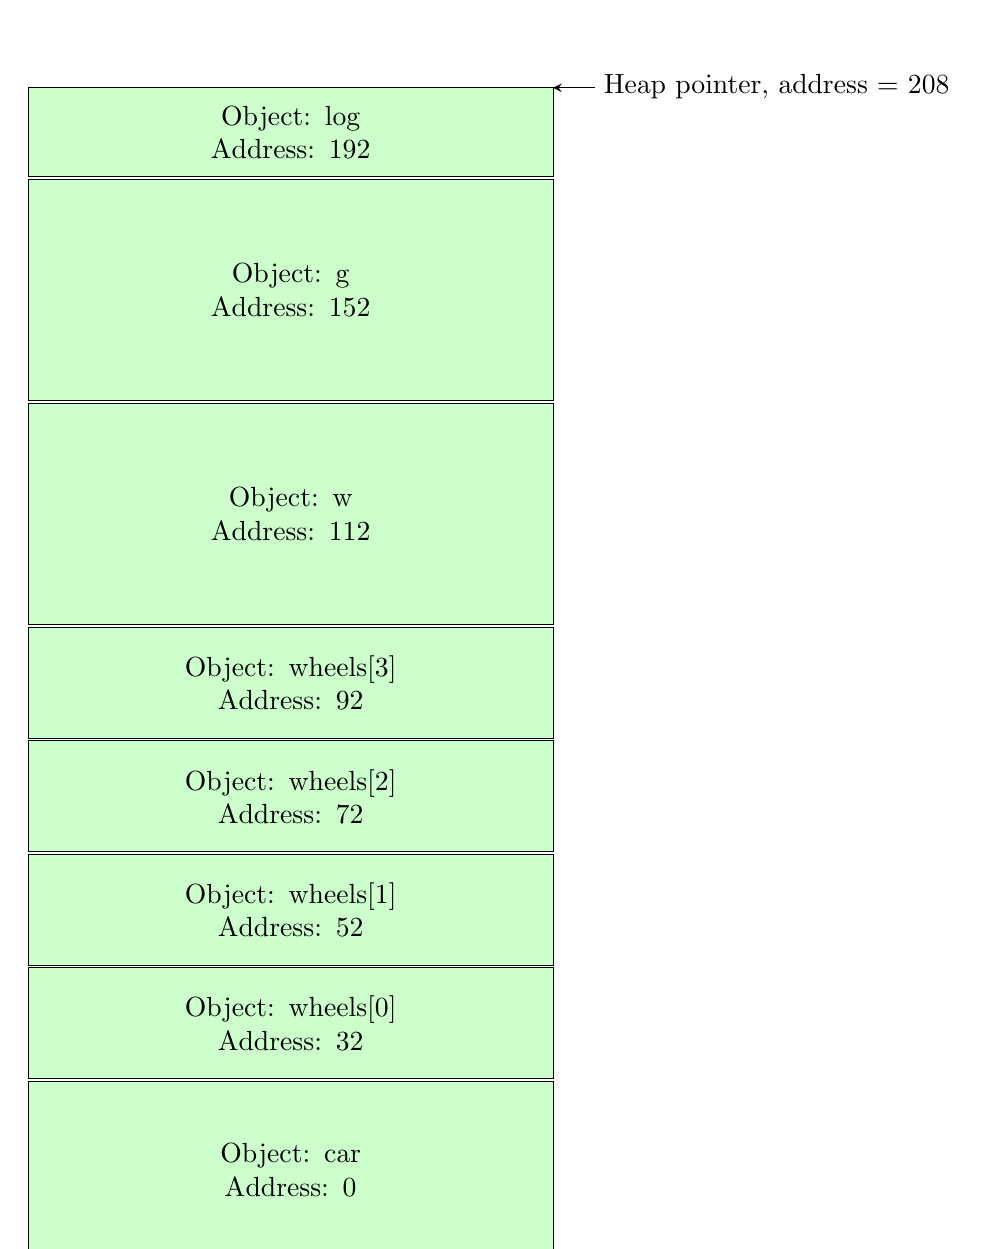
\begin{tikzpicture}[x=20pt, y=20pt, node distance=1pt,outer sep = 0pt]

\tikzstyle{box}=[rectangle,draw,anchor=north west,text centered, fill=green!20, inner sep=0.3333em]
\tikzstyle{normalbox}=[box,minimum height=32pt,text width={16em + 3*0.6666em + 3pt}]

\node[normalbox,minimum height = 32pt] (eventlog)at (1,1)  {Object: log\\Address: 192};
\node[normalbox,minimum height = 80pt] (garage) [below = of eventlog] {Object: g\\Address: 152};
\node[normalbox,minimum height = 80pt] (carwash) [below = of garage] {Object: w\\Address: 112};
\node[normalbox,minimum height = 40pt] (wheel4) [below = of carwash] {Object: wheels[3]\\Address: 92};
\node[normalbox,minimum height = 40pt] (wheel3) [below = of wheel4] {Object: wheels[2]\\Address: 72};
\node[normalbox,minimum height = 40pt] (wheel2) [below = of wheel3] {Object: wheels[1]\\Address: 52};
\node[normalbox,minimum height = 40pt] (wheel1) [below = of wheel2] {Object: wheels[0]\\Address: 32};
\node[normalbox,minimum height = 64pt] (car) [below = of wheel1] {Object: car\\Address: 0};

\draw[<-,>=stealth](eventlog.north east)--+(15pt,0) node[anchor=mid west]{Heap pointer, address = 208};
\end{tikzpicture}
\end{figure}
\end{center}

\FloatBarrier

\subsection{Copy collection during \texttt{BeginEventLoop}}

Now assume the copy garbage collection algorithm discussed in class executes during the call to BeginEventLoop. We show the state of heap memory after the first collection has concluded. Note we only show the TO space, not the FROM space (which is shown above). Additionally, we assume the TO space memory addresses begin at X. \\

In addition, we identify the root pointers and specify the order in which they were processed by the copy collection algorithm to arrive at the heap state identified. These root pointers, and their processing order are enumerated below:

\begin{enumerate}
\item We start with local variables in the \texttt{Main} stack frame, finding \texttt{car} and \texttt{log}. We copy these two objects to the TO space.
\item Next, the found \texttt{Car} object has pointers to the four \texttt{Wheel} objects (in the \texttt{wheels} list). Thus we copy these objects to the TO space.
\item The objects \texttt{w} and \texttt{g} were local to \texttt{Initialize(car)}. This function has already resolved when \texttt{BeginEventLoop} is called; hence \texttt{w} and \texttt{g} are dead. Thus they are not copied to TO space.
\end{enumerate}

The final state of TO space memory is shown in the diagram on the next page.

\begin{center}
\begin{figure}
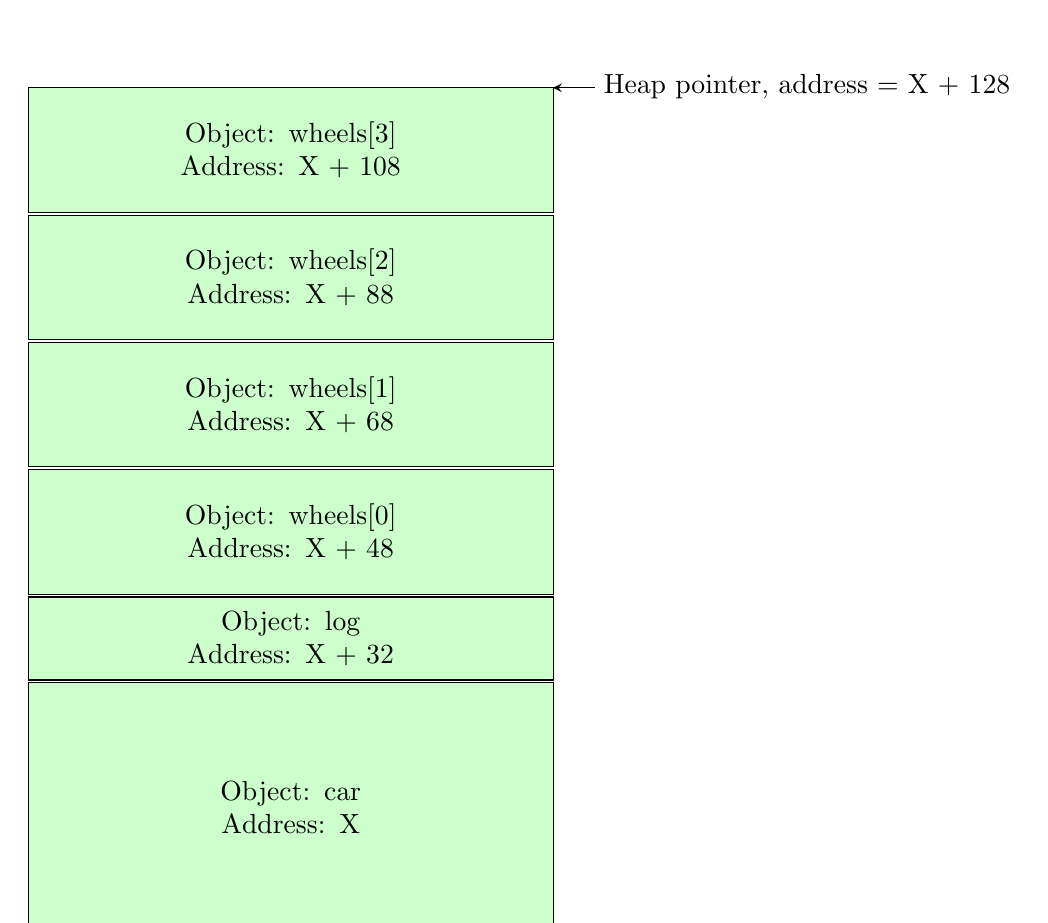
\begin{tikzpicture}[x=20pt, y=20pt, node distance=1pt,outer sep = 0pt]

\tikzstyle{box}=[rectangle,draw,anchor=north west,text centered, fill=green!20, inner sep=0.3333em]
\tikzstyle{normalbox}=[box,minimum height=30pt,text width={16em + 3*0.6666em + 3pt}]

\node[normalbox,minimum height = 45pt] (wheel4) at (1,1) {Object: wheels[3]\\Address: X + 108};
\node[normalbox,minimum height = 45pt] (wheel3) [below = of wheel4] {Object: wheels[2]\\Address: X + 88};
\node[normalbox,minimum height = 45pt] (wheel2) [below = of wheel3] {Object: wheels[1]\\Address: X + 68};
\node[normalbox,minimum height = 45pt] (wheel1) [below = of wheel2] {Object: wheels[0]\\Address: X + 48};
\node[normalbox,minimum height = 30pt] (eventlog) [below = of wheel1] {Object: log\\Address: X + 32};
\node[normalbox,minimum height = 90pt] (car) [below = of eventlog] {Object: car\\Address: X};

\draw[<-,>=stealth](wheel4.north east)--+(15pt,0) node[anchor=mid west]{Heap pointer, address = X + 128};
\end{tikzpicture}
\end{figure}
\end{center}

\FloatBarrier

\section{Prolog}

See attached .pl knowledge base and queries.

\section{Prolog Performance}

Consider the following:

\begin{lstlisting}
foo(ashwin).
foo(roberta).

hello(brock).
hello(roberta).
hello(john).

world(ashwin).
world(roberta).

goal(X) :- sub1(X),sub2(X).
sub1(X) :- foo(X).
sub2(X) :- hello(X),world(X).
\end{lstlisting}

\subsection{Faster query time for \texttt{goal(X)}}

We can provide faster execution time when querying \texttt{goal(X)} by reordering the facts as follows:

\begin{lstlisting}
foo(roberta).
foo(ashwin).


hello(roberta).
hello(brock).
hello(john).

world(roberta).
world(ashwin).

goal(X) :- sub1(X),sub2(X).
sub1(X) :- foo(X).
sub2(X) :- hello(X),world(X).
\end{lstlisting}

\subsection{Explaining why this ordering improves execution time}

Reordering the facts improves the execution time because it avoids backtracking. Under the original ordering, our knowledge base forms the following tree:

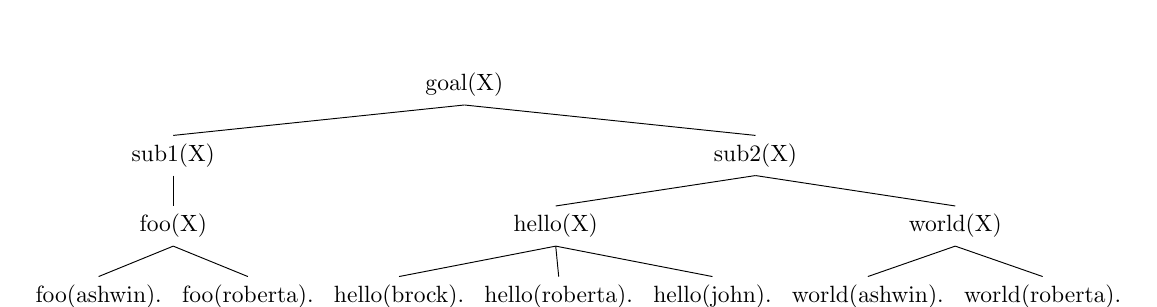
\begin{tikzpicture}[scale=.85]
\Tree [.goal(X) [.sub1(X) [.foo(X) foo(ashwin). foo(roberta). ]]
		      [.sub2(X) [.hello(X) hello(brock). hello(roberta). hello(john). ]
				     [.world(X) world(ashwin). world(roberta). ]
		      ]
	]
\end{tikzpicture}

When we query \texttt{goal(X).}, we first traverse the tree down to \texttt{foo(ashwin)}. Thus, we initially unify X and ashwin. This proceeds until \texttt{hello(ashwin)} fails, and we have to backtrack all the way to \texttt{foo(X)}, where we next try unifying X and roberta. This succeeds, but we wasted time exploring the tree with X bound to ashwin.

\begin{lstlisting}
[trace]  ?- goal(X).
   Call: (7) goal(_G2397) ? creep
   Call: (8) sub1(_G2397) ? creep
   Call: (9) foo(_G2397) ? creep
   Exit: (9) foo(ashwin) ? creep
   Exit: (8) sub1(ashwin) ? creep
   Call: (8) sub2(ashwin) ? creep
   Call: (9) hello(ashwin) ? creep
   Fail: (9) hello(ashwin) ? creep
   Fail: (8) sub2(ashwin) ? creep
   Redo: (9) foo(_G2397) ? creep
   Exit: (9) foo(roberta) ? creep
   Exit: (8) sub1(roberta) ? creep
   Call: (8) sub2(roberta) ? creep
   Call: (9) hello(roberta) ? creep
   Exit: (9) hello(roberta) ? creep
   Call: (9) world(roberta) ? creep
   Exit: (9) world(roberta) ? creep
   Exit: (8) sub2(roberta) ? creep
   Exit: (7) goal(roberta) ? creep
X = roberta.
\end{lstlisting}

In contrast, after reordering the facts, we have the following tree:

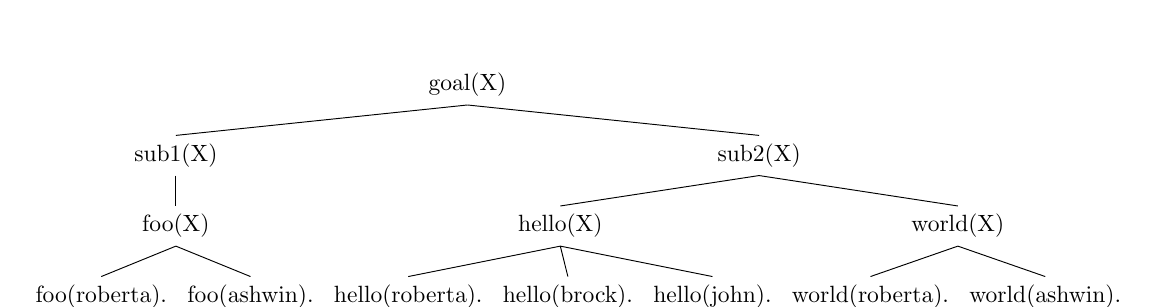
\begin{tikzpicture}[scale=.85]
\Tree [.goal(X) [.sub1(X) [.foo(X) foo(roberta). foo(ashwin). ]]
		      [.sub2(X) [.hello(X) hello(roberta). hello(brock). hello(john). ]
				     [.world(X) world(roberta). world(ashwin). ]
		      ]
	]
\end{tikzpicture}

When we query \texttt{goal(X).}, we first traverse the tree down to \texttt{foo(roberta)}. Thus, we initially unify X and roberta, and avoid having to backtrack (as this unification instantiates all the subgoals).

\begin{lstlisting}
[trace]  ?- goal(X).
   Call: (7) goal(_G2397) ? creep
   Call: (8) sub1(_G2397) ? creep
   Call: (9) foo(_G2397) ? creep
   Exit: (9) foo(roberta) ? creep
   Exit: (8) sub1(roberta) ? creep
   Call: (8) sub2(roberta) ? creep
   Call: (9) hello(roberta) ? creep
   Exit: (9) hello(roberta) ? creep
   Call: (9) world(roberta) ? creep
   Exit: (9) world(roberta) ? creep
   Exit: (8) sub2(roberta) ? creep
   Exit: (7) goal(roberta) ? creep
X = roberta .
\end{lstlisting}

\subsection{Adding break \texttt{sub1(X) :- foo(X), !}}

Now, going back to the original ordering of facts, now suppose we rewrite goal \texttt{sub1} to read: \texttt{sub1(X) :- foo(X), !}. Upon returning to query mode and querying \texttt{goal(X)}, the interpreter displays false.\\

This occurs because under the original ordering of facts, X is first bound to ashwin. Since \texttt{foo(ashwin)} is \texttt{true}, \texttt{sub1(X) :- foo(X), !} proceeds to the break "!", which prevents backtracking (i.e. binding X to roberta, such that \texttt{goal(X)} is true).

We can see this in the trace:

\begin{lstlisting}
[trace]  ?- goal(X).
   Call: (7) goal(_G2397) ? creep
   Call: (8) sub1(_G2397) ? creep
   Call: (9) foo(_G2397) ? creep
   Exit: (9) foo(ashwin) ? creep
   Exit: (8) sub1(ashwin) ? creep
   Call: (8) sub2(ashwin) ? creep
   Call: (9) hello(ashwin) ? creep
   Fail: (9) hello(ashwin) ? creep
   Fail: (8) sub2(ashwin) ? creep
   Fail: (7) goal(_G2397) ? creep
false.
\end{lstlisting}


\subsection{Adding break \texttt{sub2(X) :- hello(X), !, world(X).}}

Now, going back to the original ordering of facts, now suppose we rewrite goal \texttt{sub2} to read: \texttt{sub2(X) :- hello(X), !, world(X).}. Upon returning to query mode and querying \texttt{goal(X)}, this time the goal succeeds.\\

This is because the break is \textbf{not} reached until X is bound to roberta. Initially, X is bound to ashwin. However, when we reach \texttt{sub2}, \texttt{hello(ashwin)} fails and ! is not reached. Instead, we backtrack all the way to the subgoal \texttt{sub1(X) :- foo(X)}, and bind X to roberta. Thus, the break is not reached until X is bound to roberta, which is fine since world(roberta) is true.

To see this more clearly, we show the trace for a modified version of this rule- the modified version is:\\
\texttt{sub2(X) :- hello(X), write("Before break"), !, write("After break"), world(X).}\\

The trace for this modified version is shown below.

\begin{lstlisting}
[trace]  ?- goal(X).
   Call: (7) goal(_G2397) ? creep
   Call: (8) sub1(_G2397) ? creep
   Call: (9) foo(_G2397) ? creep
   Exit: (9) foo(ashwin) ? creep
   Exit: (8) sub1(ashwin) ? creep
   Call: (8) sub2(ashwin) ? creep
   Call: (9) hello(ashwin) ? creep
   Fail: (9) hello(ashwin) ? creep
   Fail: (8) sub2(ashwin) ? creep
   Redo: (9) foo(_G2397) ? creep
   Exit: (9) foo(roberta) ? creep
   Exit: (8) sub1(roberta) ? creep
   Call: (8) sub2(roberta) ? creep
   Call: (9) hello(roberta) ? creep
   Exit: (9) hello(roberta) ? creep
   Call: (9) write("Before break") ? creep
Before break
   Exit: (9) write("Before break") ? creep
   Call: (9) write("After break") ? creep
After break
   Exit: (9) write("After break") ? creep
   Call: (9) world(roberta) ? creep
   Exit: (9) world(roberta) ? creep
   Exit: (8) sub2(roberta) ? creep
   Exit: (7) goal(roberta) ? creep
X = roberta.
\end{lstlisting}

Clearly we don't reach the break (which is bound by \texttt{write("Before break")} and \texttt{write("After break")}) until we've rebound X to roberta. 

\section{Unification}

\subsection{d(15) \& c(X)}

This pair does not unify, since the constants d and c differ. and constants only unify with themselves.

\subsection{a(X, b(3, 1, Y)) \& a(4, Y)}

This pair does not unify, since the second argument to the functor a would need to unify, but Y cannot unify with b(3,1, y), since this yields an infinite recursion.

\subsection{a(X, c(2, B, D)) \& a(4, c(A, 7, C))}

This pair does unify, with the following bindings:
\begin{itemize}
\item X = 4,
\item A = 2,
\item B = 8
\item C = D
\end{itemize}

\subsection{a(X, c(2, A, X)) \& a(4, c(A, 7, C))}

This pair does not unify, since we would obtain the following contradictory bindings:
\begin{itemize}
\item X = 4,
\item A = 2 and 7 (\textbf{contradiction}!),
\item C = 4,
\end{itemize}

\subsection{e(c(2,D)) \& e(c(8, D))}

This pair does not unify, since the constants 2 and 8 differ, and constants only unify with themselves.

\subsection{X \& e(f(6,2), g(8, 1))}

This pair does unify, with the binding
\begin{itemize}
\item X = e(f(6,2), g(8, 1))
\end{itemize}

\subsection{b(X, g(8, X)) \& b(f(6,2), g(8, f(6,2)))}

This pair does unify, with the binding
\begin{itemize}
\item X = f(6,2)
\end{itemize}

\subsection{a(1, b(X, Y)) \& a(Y, b(2, c(6, Z), 10))}

This pair does not unify for  a number of reasons, primarily because b/2 and b/3 can't unify since they differ in arity. 

\subsection{d(c(1,2,1)) \& d( c(X, Y, X))}

This pair does unify, with the bindings
\begin{itemize}
\item X = 1
\item Y = 2
\end{itemize}


%----------------------------------------------------------------------------------------
\end{document}